%fich.tex
%%%%%%%%%%%%%%%%%%%%%%%%%%%%%%%%%%%%%%%%%%%%%%%%%%%%%%%%%%%%%%%%%%%%%%%%
% Manuel González Pérez
% Descripción del documento:
	
%%%%%%%%%%%%%%%%%%%%%%%%%%%%%%%%%%%%%%%%%%%%%%%%%%%%%%%%%%%%%%%%%%%%%%%%


%%%%%%%%%%%%%%%%%%%%%%%%%%%%%%%%%%%%%%%%%%%%%%%%%%%%%%%%%%%%%%%%%%%%%%%%
%Clase de documento
\documentclass[12pt, spanish]{article}
%%%%%%%%%%%%%%%%%%%%%%%%%%%%%%%%%%%%%%%%%%%%%%%%%%%%%%%%%%%%%%%%%%%%%%%%


%%%%%%%%%%%%%%%%%%%%%%%%%%%%%%%%%%%%%%%%%%%%%%%%%%%%%%%%%%%%%%%%%%%%%%%%	
%Paquetes de lenguaje:
%%%%%%%%%%%%%%%%%%%%%%%%%%%%%%%%%%%%%%%%%%%%%%%%%%%%%%%%%%%%%%%%%%%%%%%%
\usepackage[utf8]{inputenc}
\usepackage[spanish]{babel}
\usepackage{graphicx}
%\usepackage[spanish, activeacute] {babel}	
%\usepackage[spanish]{babel} 				
%\usepackage[latin1]{inputenc}
%%%%%%%%%%%%%%%%%%%%%%%%%%%%%%%%%%%%%%%%%%%%%%%%%%%%%%%%%%%%%%%%%%%%%%%%


%%%%%%%%%%%%%%%%%%%%%%%%%%%%%%%%%%%%%%%%%%%%%%%%%%%%%%%%%%%%%%%%%%%%%%%%
%Paquetes para encabezados y pie de páginas
%%%%%%%%%%%%%%%%%%%%%%%%%%%%%%%%%%%%%%%%%%%%%%%%%%%%%%%%%%%%%%%%%%%%%%%%
\usepackage{fancyhdr}
%%%%%%%%%
% \pagestyle{fancy} %Si se cambia el estilo de página, antes de empezar 
	%el documento. Esto hace que el emcabezado y pie de página se 
	%quede separado del texto por una línea
%%%%%%%%%	
% \fancyhead{} % Límpia el texto que se está usando como encabezado
%%%%%%%%%
% \fancyhead[OPCIONES]{Encabezado}
	% OPCIONES:
		% L texto a la izquierda
		% C texto centrado
		% R texto a la derecha
		% E página par
		% O pagina impar
	%Ejemplo: 
		% fancyhead [LE] {"Doc. Latex"} 
			% Establece como emcabezado de las páginas pares "Doc Latex"
			% con alineacion a la izquierda
%%%%%%%%%			
% \fancyfoot[OPCIONES]{Píe de pag.}
	% OPCIONES:
		% L C R E O
	%Ejemplo
		% \fancyfoot[LE,RO]{\thepage} 
			% Establece como píe de pág. el número de página. con 
			% alineación a la izq en paginas pares y a la derecha en
			% las impares
%%%%%%%%%			
% \renewcommand{\headrulewidth}{0.4pt}
% \renewcommand{\footrulewidth}{0.4pt}
	% Fija el grosor de la la linea que separa el emcabezado y pie de pág
%%%%%%%%%
% Otros comandos:
%\lhead{}
%\chead{}
%\rhead{}
%\lfoot{}
%\cfoot{}
%%%%%%%%%%%%%%%%%%%%%%%%%%%%%%%%%%%%%%%%%%%%%%%%%%%%%%%%%%%%%%%%%%%%%%%%


%%%%%%%%%%%%%%%%%%%%%%%%%%%%%%%%%%%%%%%%%%%%%%%%%%%%%%%%%%%%%%%%%%%%%%%%
% Paquetes para tamaños y distancias
%%%%%%%%%%%%%%%%%%%%%%%%%%%%%%%%%%%%%%%%%%%%%%%%%%%%%%%%%%%%%%%%%%%%%%%%
\usepackage{anysize} 
%%%%%%%%%%%
% \marginsize{3cm}{2cm}{2cm}{2cm}
	% Controla los márgenes {izquierda}{derecha}{arriba}{abajo}. 
%%%%%%%%%%%%%%%%%%%%%%%%%%%%%%%%%%%%%%%%%%%%%%%%%%%%%%%%%%%%%%%%%%%%%%%%


%%%%%%%%%%%%%%%%%%%%%%%%%%%%%%%%%%%%%%%%%%%%%%%%%%%%%%%%%%%%%%%%%%%%%%%%
%Paquetes de carácteres especiales:
%%%%%%%%%%%%%%%%%%%%%%%%%%%%%%%%%%%%%%%%%%%%%%%%%%%%%%%%%%%%%%%%%%%%%%%%
%\usepackage{dsfont}	
%Para representar conjuntos matematicos comunes: Z, N, R...
	% mathds{R}, mathds{N},...
%%%%%%%%%%%%%%%%%%%%%%%%%%%%%%%%%%%%%%%%%%%%%%%%%%%%%%%%%%%%%%%%%%%%%%%%


%%%%%%%%%%%%%%%%%%%%%%%%%%%%%%%%%%%%%%%%%%%%%%%%%%%%%%%%%%%%%%%%%%%%%%%%
%Paquetes de color:
%%%%%%%%%%%%%%%%%%%%%%%%%%%%%%%%%%%%%%%%%%%%%%%%%%%%%%%%%%%%%%%%%%%%%%%%
\usepackage{color}
%%%%%%%%%%%%%%%%%%%%%%%%%%%%%%%%%%%%%%%%%%%%%%%%%%%%%%%%%%%%%%%%%%%%%%%%
%Definición de colores:
\definecolor{gray97}{gray}{.97}
\definecolor{gray75}{gray}{.75}
\definecolor{gray45}{gray}{.45}
%%%%%%%%%%%%%%%%%%%%%%%%%%%%%%%%%%%%%%%%%%%%%%%%%%%%%%%%%%%%%%%%%%%%%%%%


%%%%%%%%%%%%%%%%%%%%%%%%%%%%%%%%%%%%%%%%%%%%%%%%%%%%%%%%%%%%%%%%%%%%%%%%
%Paquete de listado de código:
%%%%%%%%%%%%%%%%%%%%%%%%%%%%%%%%%%%%%%%%%%%%%%%%%%%%%%%%%%%%%%%%%%%%%%%%
\usepackage{listings}
%%%%%%%%%%%%%%%%%%%%%%%%%%%%%%%%%%%%%%%%%%%%%%%%%%%%%%%%%%%%%%%%%%%%%%%%
%Configuración del listado:
\lstset { 
	frame=Ltb,
     framerule=0pt,
     aboveskip=0.1cm,
     framextopmargin=0.3pt,
     framexbottommargin=0.2pt,
     framexleftmargin=0.3cm,
     framesep=0pt,
     rulesep=.2pt,
     backgroundcolor=\color{gray97},
     rulesepcolor=\color{black},
     %
     stringstyle=\ttfamily,
     showstringspaces = false,
     basicstyle=\small\ttfamily,
     commentstyle=\color{gray45},
     keywordstyle=\bfseries,
   	%
     numbers=left,
     numbersep=1pt,
     numberstyle=\tiny,
     numberfirstline = false,
     breaklines=true,
}
%%%%%%%%%%%%%%%%%%%%%%%%%%%%%%%%%%%%%%%%%%%%%%%%%%%%%%%%%%%%%%%%%%%%%%%%


%%%%%%%%%%%%%%%%%%%%%%%%%%%%%%%%%%%%%%%%%%%%%%%%%%%%%%%%%%%%%%%%%%%%%%%%
%Estilo de página
%%%%%%%%%%%%%%%%%%%%%%%%%%%%%%%%%%%%%%%%%%%%%%%%%%%%%%%%%%%%%%%%%%%%%%%%
%\textwidth 6.75in								  %ancho de texto
%\oddsidemargin -0.2in							%margen izquierdo 
\parskip 0.2in									%espacio parrafos
%%%%%%%%%%%%%%%%%%%%%%%%%%%%%%%%%%%%%%%%%%%%%%%%%%%%%%%%%%%%%%%%%%%%%%%%


%%%%%%%%%%%%%%%%%%%%%%%%%%%%%%%%%%%%%%%%%%%%%%%%%%%%%%%%%%%%%%%%%%%%%%%%	
%datos del documento
%\title{Estudio Dietético Programado 2011\\Manual de Usuario}						%titulo
%\author{Manuel González Pérez}						%autor
%\date{}												%fecha
%%%%%%%%%%%%%%%%%%%%%%%%%%%%%%%%%%%%%%%%%%%%%%%%%%%%%%%%%%%%%%%%%%%%%%%%


%%%%%%%%%%%%%%%%%%%%%%%%%%%%%%%%%%%%%%%%%%%%%%%%%%%%%%%%%%%%%%%%%%%%%%%%
%Documento:
%%%%%%%%%%%%%%%%%%%%%%%%%%%%%%%%%%%%%%%%%%%%%%%%%%%%%%%%%%%%%%%%%%%%%%%%
\begin{document}
%%%%%%%%%%%%%%%%%%%%%%%%%%%%%%%%%%%%%%%%%%%%%%%%%%%%%%%%%%%%%%%%%%%%%%%%
%\maketitle
%\newpage
%\pagebreak 
\tableofcontents
\newpage
\section{Introducción}
Este manual pretende ser una guía para la correcta utilización del programa
de escritorio Estudio Dietético Programado 2011 (EDP11).
Este programa es un software para la realización de dietas personalizadas así
como el seguimiento del paciente en su evolución.
\newpage


\section{Presentación de la aplicación}
La aplicación esta orientada a dietistas profesionales con el fin de poder dar un buen servicio y seguimiento de sus pacientes.
Cuando el usuario inicia la aplicación se mostrará la pantalla principal de la misma. Desde ella se podrá acceder a las diferentes opciones ofrecidas, descritas a lo largo de este manual.
La aplicación contiene los siguientes componentes:
\begin{itemize}
\item \textbf{Barra de menú superior:} En dicha barra se mostrarán las distintas acciones posibles, habilitándose y deshabilitándose según la ejecución de la aplicación.
\item \textbf{Área de información rápida:} En dicha área se podrán observar el nombre, edad, peso actual y peso objetivo, así como un icono de información que determinará si hay información relevante para el tratamiento del paciente.
\item \textbf{Pestañas interiores de información e interactuación:} En dichas pestañas se obtendrán información del paciente a tratar así como aquello con lo que se pueda interactuar, separados en \textbf{Datos Personales}, \textbf{Estudio Antropométrico}, \textbf{Historia Dietética} y \textbf{Registro Dietético}
\end{itemize}
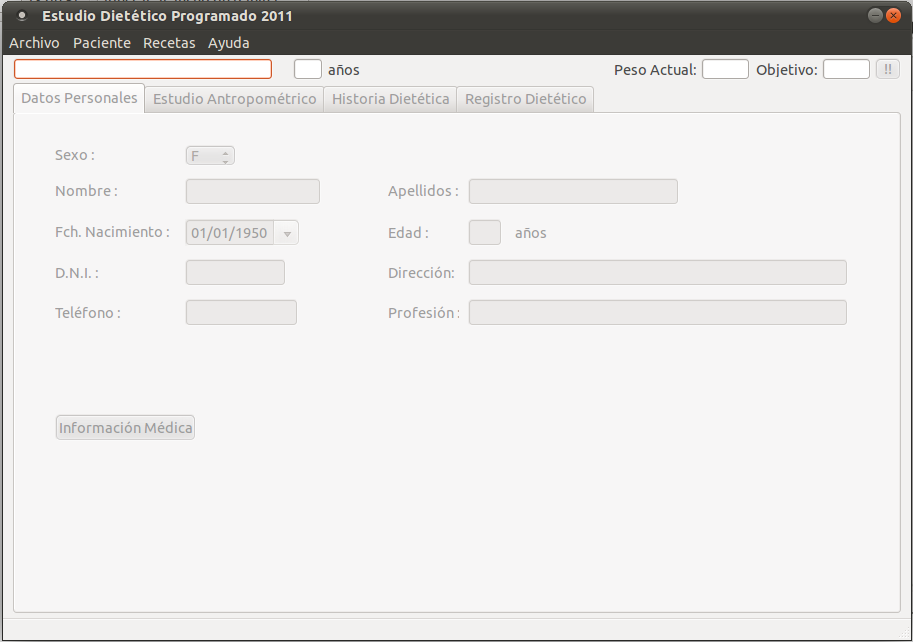
\includegraphics[scale=0.5]{Image/aplicacion.png} 
\newpage


\subsection{Barra de menú superior}

\includegraphics[scale=0.5]{Image/barra-superior.png}\\\\
La barra superior contiene los submenús:
\begin{itemize}
\item Archivo
\begin{itemize}
\item Abrir Perfil Dietista
\item Cerrar Perfil
\item Guardar
\item Imprimir
\item Salir
\end{itemize}
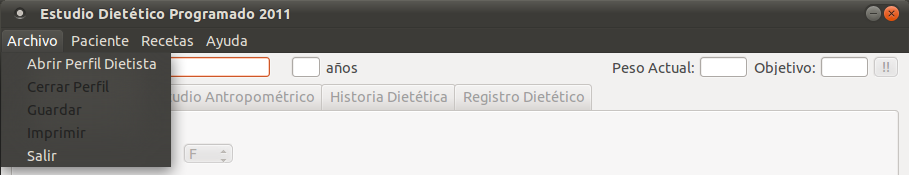
\includegraphics[scale=0.5]{Image/archivo-barra.png} 
\item Paciente
\begin{itemize}
\item Nuevo Paciente
\item Abrir Paciente
\item Cerrar Paciente
\item Eliminar Paciente
\end{itemize}
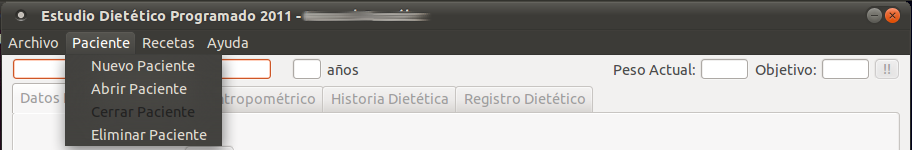
\includegraphics[scale=0.5]{Image/paciente-barra.png} 
\item Recetas
\begin{itemize}
\item Nueva Receta
\item Editar Receta
\item Eliminar Receta
\end{itemize}
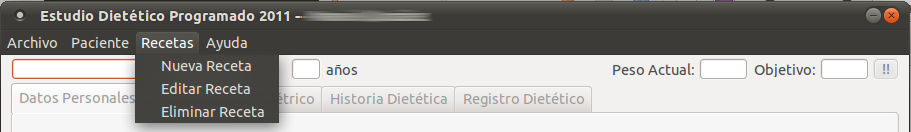
\includegraphics[scale=0.5]{Image/receta-barra.png} 
\item Ayuda
\begin{itemize}
\item Manual
\item Acerca de
\end{itemize}
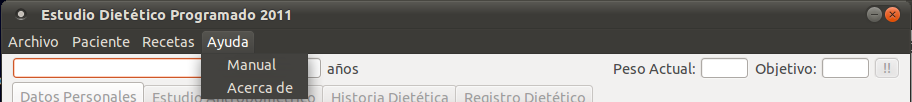
\includegraphics[scale=0.5]{Image/ayuda-barra.png} 
\end{itemize}



\subsubsection{Archivo}
\begin{enumerate}
\item \textbf{Abrir Perfil Dietista:}\\\\
Desde aquí se podrá seleccionar el perfil de dietista a abrir, así como crear un perfil nuevo o eliminar uno existente.\\\\
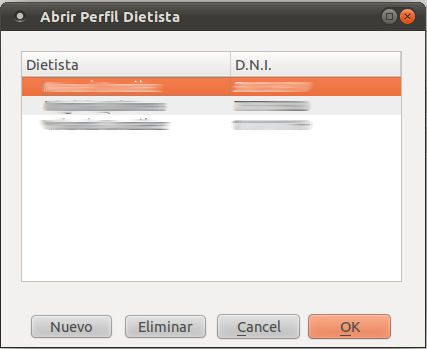
\includegraphics[scale=0.5]{Image/dietista-abrir.png}
\begin{enumerate}
\item \textit{Seleccionar perfil existente.}\\\\
Al seleccionar un perfil existente se pasará a la ventana de contraseña, en la cual habrá que introducir la contraseña correspondiente al perfil.\\\\
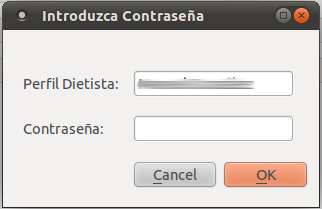
\includegraphics[scale=0.5]{Image/dietista-passwd.png}
\item \textit{Nuevo Perfil.}\\\\
Al seleccionar Nuevo se podrá incluir un nuevo perfil en el cual tendremos que rellenar los datos correspondientes así como elegir una contraseña para próximas insercciones.\\\\
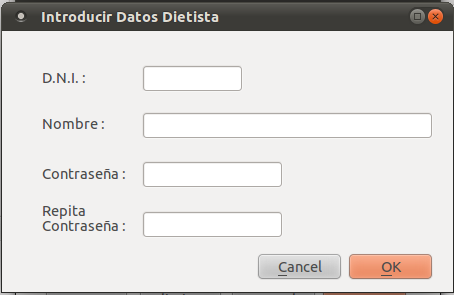
\includegraphics[scale=0.5]{Image/dietista-datos.png}
\item \textit{Eliminar Perfil.}\\\\
Si procede a eliminar un perfil existente accederá a la ventana de confirmación, en tal caso deberá introducir la clave de administración, la cual deberá solicitar al administrador (gonzalezperezmanuel@gmail.com)\\\\
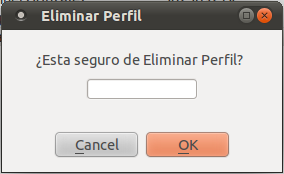
\includegraphics[scale=0.5]{Image/dietista-eliminar.png}
\end{enumerate}
\item \textbf{Cerrar Perfil:}\\\\
Al seleccionar Cerrar Perfil se cerrará el perfil en ejecución actual.\\\\
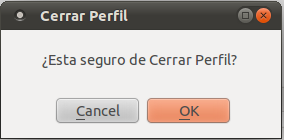
\includegraphics[scale=0.5]{Image/dietista-cerrar.png}
\item \textbf{Guardar}\\\\
Al seleccionar Guardar se guardarán los cambios efectuados a lo largo del programa.
\item \textbf{Imprimir}\\\\
Al seleccionar Imprimir se imprimirá el semanario último guardado, así como las correspondientes elaboraciones de cada plato.\\\\
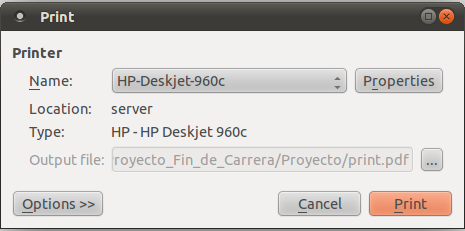
\includegraphics[scale=0.5]{Image/dietista-imprimir.png}
\item \textbf{Salir}\\\\
Al seleccionar Salir se saldrá de la aplicación.\\\\
\end{enumerate}
\newpage





\subsubsection{Paciente}
\begin{enumerate}
\item \textbf{Nuevo Paciente}\\\\
Al seleccionar Nuevo Paciente se podrá dar de alta a un paciente asociado al perfil de dietista actual.\\\\
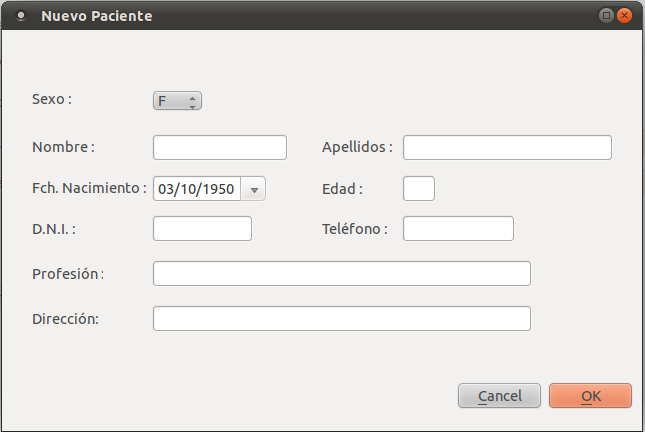
\includegraphics[scale=0.5]{Image/paciente-nuevo1.png}\\\\
Una vez introducidos los datos, se pasará a la siguiente ventana.\\\\
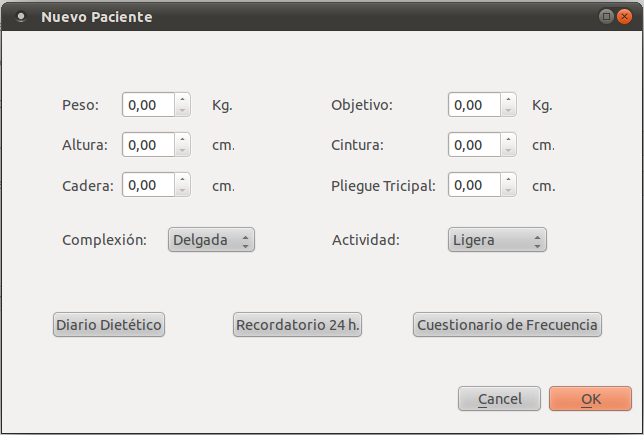
\includegraphics[scale=0.5]{Image/paciente-nuevo2.png}\\\\
Desde esta ventana se podrá imprimir el \textit{Diario Dietético} y el \textit{Recordatorio 24 h.}; así como rellenar el \textit{Cuestionario de Frecuencia}.
\begin{enumerate}
\item \textit{Diario Dietético.}\\\\
El Diario Dietético se trata de un diario de 3 días el cual el paciente se deberá llevar a casa para rellenarlo siguiendo las instrucciones, apuntando todas las comidas que hace durante los días señalados.
\item \textit{Recordatorio 24 h.}\\\\
El Recordatorio 24 h. se trata de un diario de 1 día el cual el paciente deberá rellenar con lo que recuerde haber comido en el día anterior.
\item \textit{Cuestionario de Frecuencia.}\\\\
El Cuestionario de Frecuencia servirá para apuntar la frecuencia con la cual se consumen los alimentos, así como la preferencia puntuando de 1 a 5 sobre los mismos.\\\\
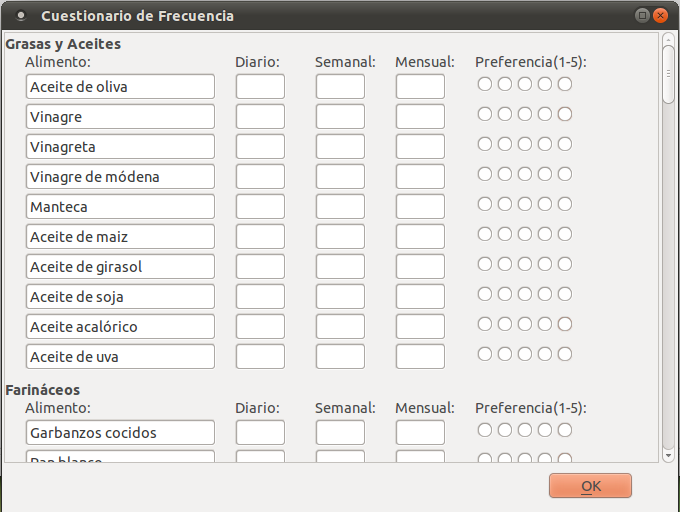
\includegraphics[scale=0.5]{Image/cuestfrec.png}\\\\
\end{enumerate}
\item \textbf{Abrir Paciente}\\\\
Al seleccionar Abrir Paciente se accederá a la ventana con el listado de los pacientes del dietista actual. Desde aquí se podrá seleccionar al paciente deseado.\\\\
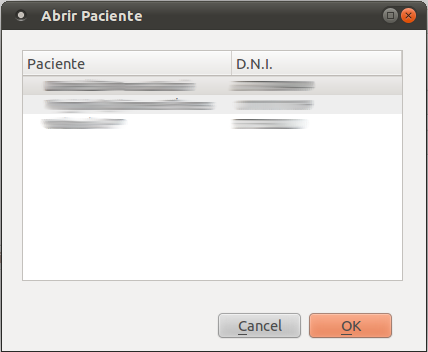
\includegraphics[scale=0.5]{Image/paciente-abrir.png}\\\\
\item \textbf{Cerrar Paciente}\\\\
Desde aquí se cerrará el perfil de paciente actual.\\
\item \textbf{Eliminar Paciente}\\\\
Desde aquí se accederá al listado de pacientes, desde el cual se podrá eliminar el paciente seleccionado y así todos sus datos.\\\\
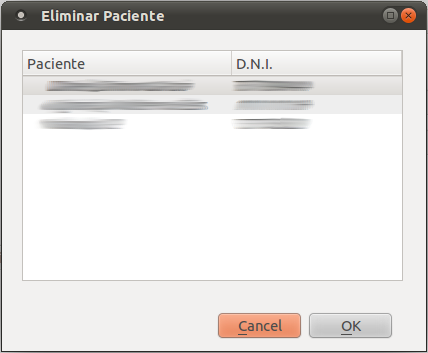
\includegraphics[scale=0.5]{Image/paciente-eliminar.png}\\\\
\end{enumerate}
\newpage





\subsubsection{Recetas}
\begin{enumerate}
\item \textbf{Nueva Receta}\\\\
Al seleccionar Nueva Receta se accederá a la ventana desde la cual elaborar una nueva receta perteneciente al perfil del dietista actual.\\\\
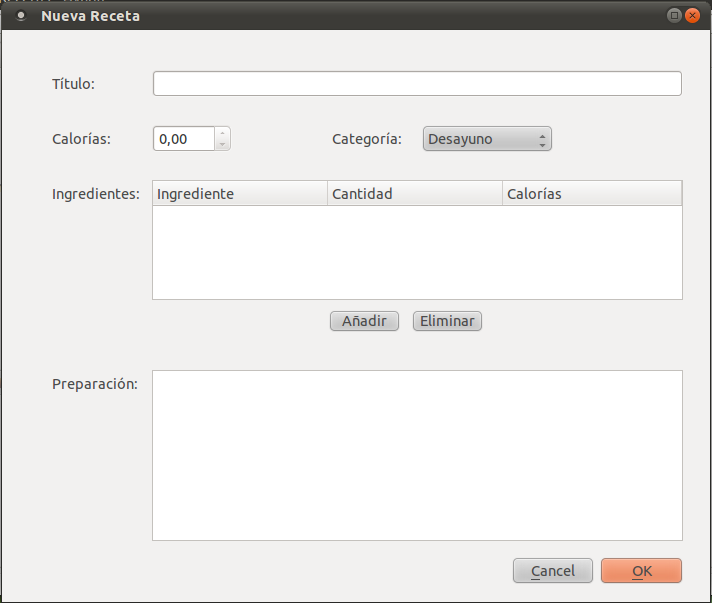
\includegraphics[scale=0.5]{Image/receta-nueva.png}\\\\
En la elaboración de la receta se rellenará el nombre, los ingredientes y las indicaciones para la preparación. 
\begin{enumerate}
\item \textit{Añadir Ingredientes}\\\\
Para añadir ingredientes se seleccionará Añadir, el cual accederá a la ventana de selección de ingredientes.\\\\
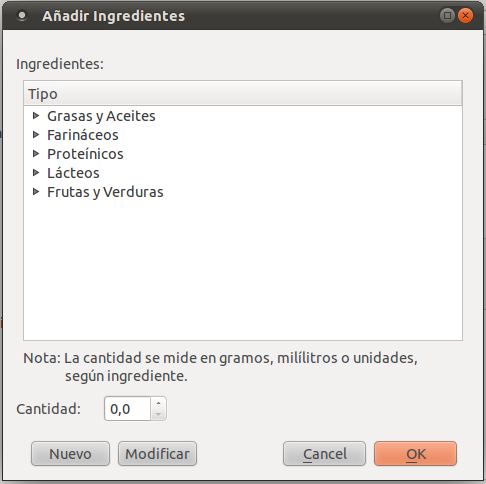
\includegraphics[scale=0.5]{Image/ingrediente-anadir.png}\\\\
Estos ingredientes estarán clasificados por grupos y alfabeticamente, ofreciendo una mejora en la búsqueda.
Desde aquí se podrá seleccionar el ingrediente y escribir la cantidad deseada para la receta.
En el caso de no encontrar un ingrediente u observar alguna errata en alguno de ellos, existen opciones para las operaciones respectivamente.\\\\
\begin{enumerate}
\item \textit{Nuevo}\\\\
Al seleccionar Nuevo, se accederá a la ventana desde la cual describir todo lo necesario para ingresar un nuevo ingrediente.\\\\
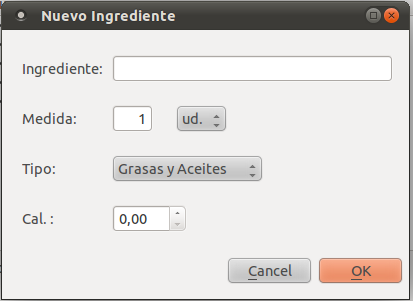
\includegraphics[scale=0.5]{Image/ingrediente-nuevo.png}\\\\
En dicha ventana se pedirá nombre del ingrediente, medida en la que se medirá, pudiendo ser 1, 10, 100 siendo unidad, mililitros y gramos respectivamente, tipo, donde se pondrá el grupo al que pertenece, y por último las calorías del ingrediente que comprenden la medida elegida.
\item \textit{Modificar}\\\\
Al seleccionar un ingrediente y posteriormente la opción Modificar, se podrá modificar cualquiera de los campos del ingrediente.\\\\
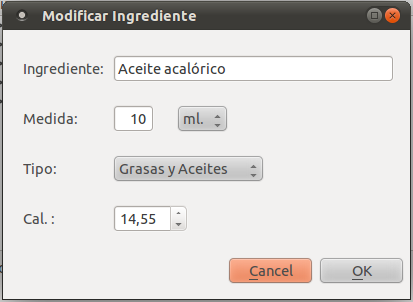
\includegraphics[scale=0.5]{Image/ingrediente-modificar.png}\\\\
Atención: Al modificar un ingrediente, quedarán modificadas todas las recetas en las que aparezca dicho ingrediente. Se recomienda revisarlas para evitar errores con respecto a las calorías.\\\\
\end{enumerate}
\item \textit{Eliminar Ingredientes}\\\\
Al seleccionar Eliminar se eliminará el ingrediente seleccionado de la lista de ingredientes que componen la receta.\\\\
\end{enumerate}
\item \textbf{Editar Receta}\\\\
Al seleccionar Editar Receta, se obtendrá un listado con todas las recetas.\\\\
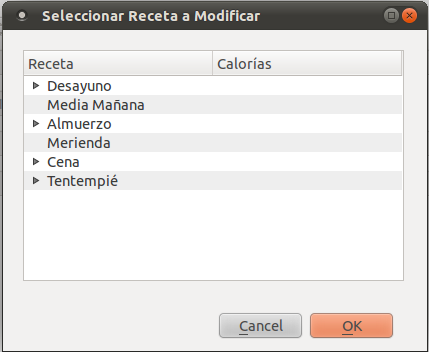
\includegraphics[scale=0.5]{Image/receta-modificar.png}\\\\
Desde aquí se elegirá una de las recetas para su modificación, obteniendo todos los datos, puediendo modificar cualquiera de los campos.\\\\
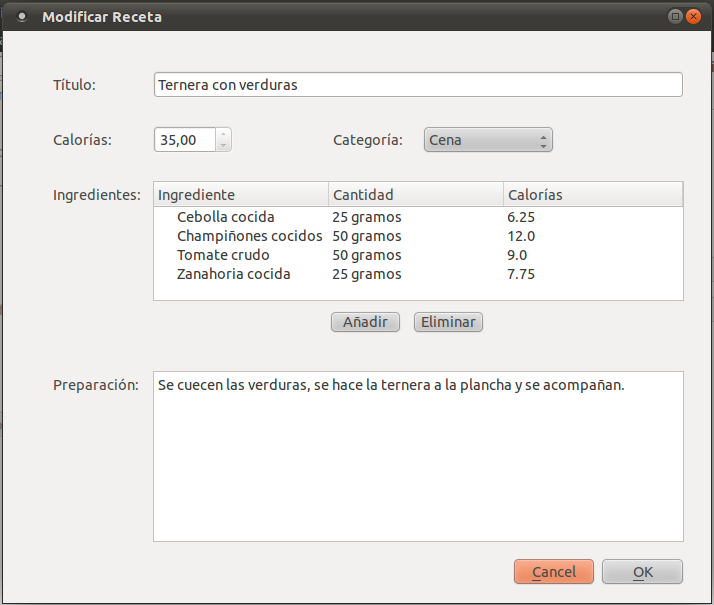
\includegraphics[scale=0.5]{Image/receta-modificar2.png}\\\\
Nótese que existen las opciones Añadir y Eliminar, las cuales tendrán las mismas funciones que las accesibles desde la opción Nueva Receta
\item \textbf{Eliminar Receta}\\\\
Al seleccionar Eliminar Receta se obtendrá un listado de las recetas ordenadas igualmente por tipo de receta y alfabéticamente, de las cuales seleccionar cual se desea eliminar.\\\\
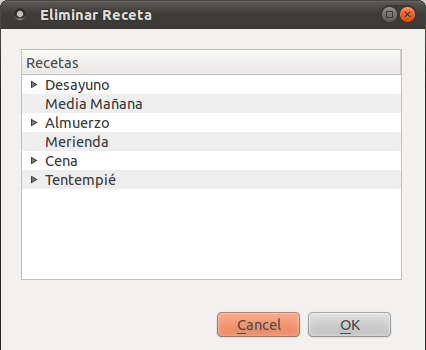
\includegraphics[scale=0.5]{Image/receta-eliminar.png}
\end{enumerate}
\newpage



\subsubsection{Ayuda}
\begin{enumerate}
\item \textbf{Manual}\\\\
Al seleccionar Manual se accederá al presente manual.\\
\item \textbf{Acerca de}\\\\
Al seleccionar Acerca de, se accederá a la ventana que ofrece información sobre la aplicación.\\\\
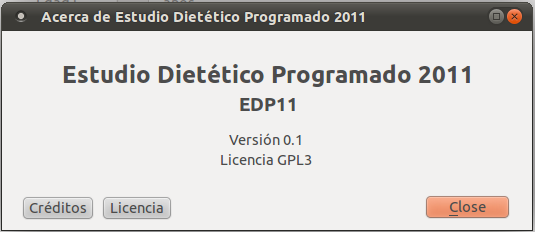
\includegraphics[scale=0.5]{Image/acercade.png}\\\\
Desde aquí también se podrá acceder a los Créditos y a la Licencia.\\
\begin{enumerate}
\item \textit{Créditos}\\\\
Seleccionando Créditos podrá acceder a la ventana de información acerca de la realización y soporte de la aplicación.\\\\
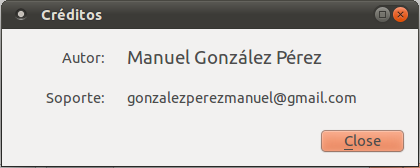
\includegraphics[scale=0.5]{Image/creditos.png}\\\\
\item \textit{Licencia}\\\\
Seleccionando Licencia se accederá a los términos de la Licencia bajo la que se distribuye la aplicación, siendo en este caso GPL3.0.\\\\
\end{enumerate}
\end{enumerate}


\subsection{Pestañas interiores de información e interactuación}
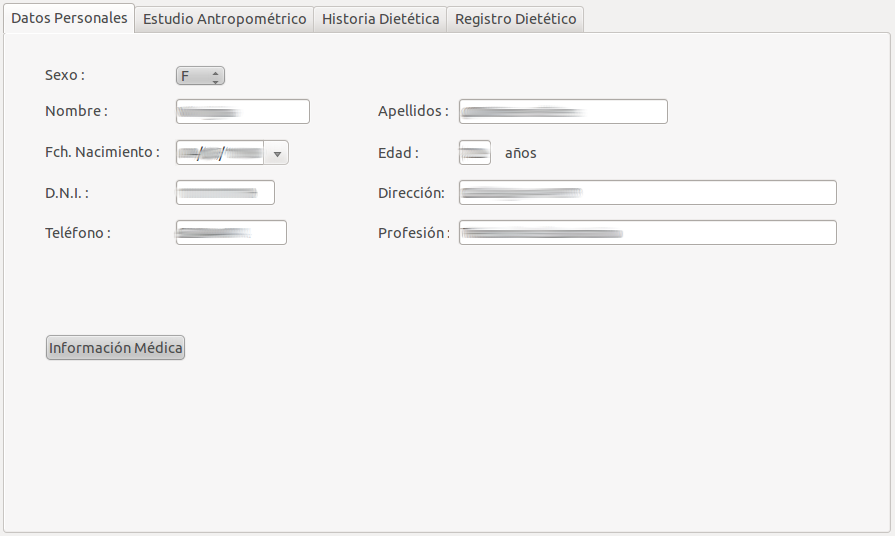
\includegraphics[scale=0.5]{Image/pestanas.png}\\\\
A través de las pestañas es desde donde se presentarán los datos del paciente, y desde donde se le realizará el seguimiento.
Se compone de cuatro pestañas:
\begin{itemize}
\item Datos Personales
\item Estudio Antropométrico
\item Historia Dietética
\item Registro Dietético
\end{itemize}
\newpage


\subsubsection{Datos Personales}
Desde aquí se mostrarán los datos personales del paciente, tales como sexo, nombre, apellidos, fecha de nacimiento, edad, dni, dirección, teléfono y profesión.\\\\
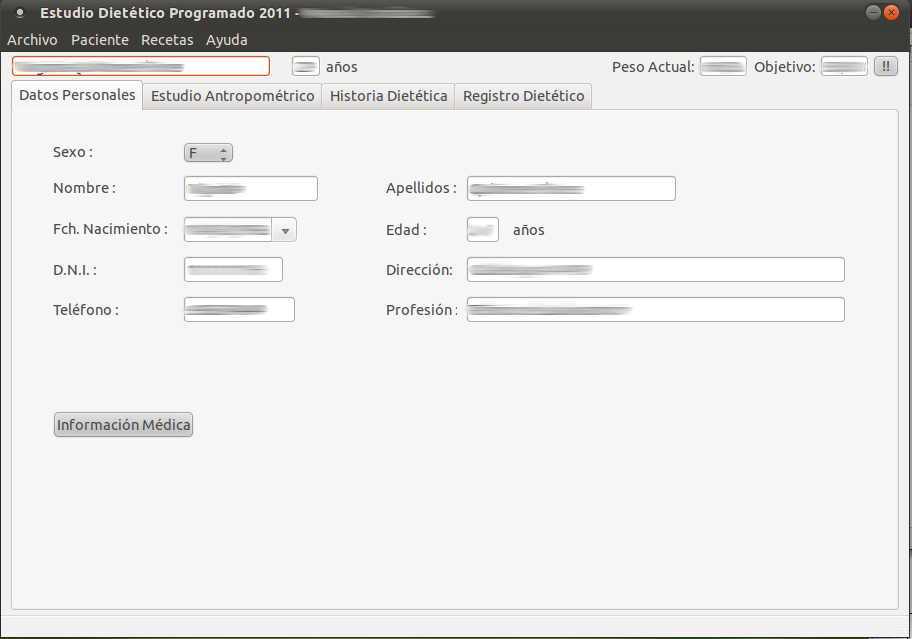
\includegraphics[scale=0.5]{Image/paciente-datos.png}\\\\
También se podrá acceder a Información Médica relevante.
\begin{enumerate}
\item \textit{Información Médica}\\\\
Al seleccionar Información Médica se accederá a datos relevantes sobre el paciente, como análíticas, tratamiento farmacológico, y también enfermedades y patologías.\\\\
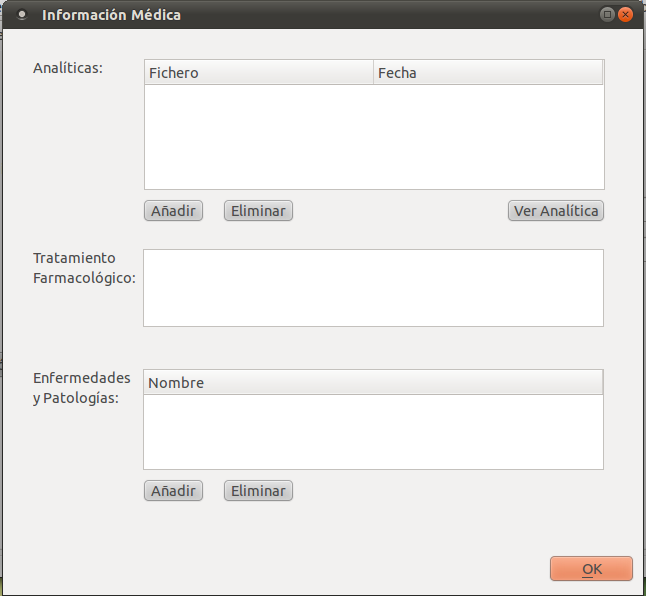
\includegraphics[scale=0.5]{Image/infomed.png}\\\\
\begin{enumerate}
\item Analíticas\\\\
En la sección de analíticas se mostrarán las analíticas del paciente que se realice a lo largo de su seguimiento.
\begin{enumerate}
\item Añadir\\\\
Al seleccionar Añadir, se abrirá un diálogo para seleccionar el PDF escaneado de la analítica.\\
\item Eliminar\\\\
Al seleccionar Eliminar, se eliminará el análisis seleccionado.\\
\item Ver Analítica\\\\
Al seleccionar Ver Analítica, se abrirá el PDF de la analítica seleccionado.\\
\end{enumerate}
\item Tratamiento Farmacológico\\\\
En tratamiento farmacológico describirá cualquier tipo de medicación del paciente, la cual se deba tener en cuenta o pueda influir en el seguimiento del mismo.\\
\item Enfermedades y Patologías\\\\
En enfermedades y patologías se mostrarán las enfermedades o patologías que tenga el paciente.\\
\begin{enumerate}
\item Añadir\\\\
Al seleccionar Añadir, se abrirá un listado con las distintas enfermedades o patologías registradas.\\\\
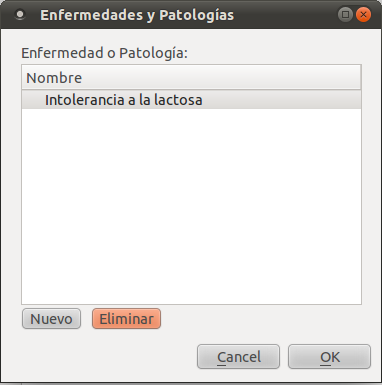
\includegraphics[scale=0.5]{Image/enfermedad.png}\\\\
\begin{enumerate}
\item Nuevo\\\\
En el caso de no encontrar la enfermedad o patología deseada, se podrá registrar una nueva, seleccionando la opción Nuevo.\\\\
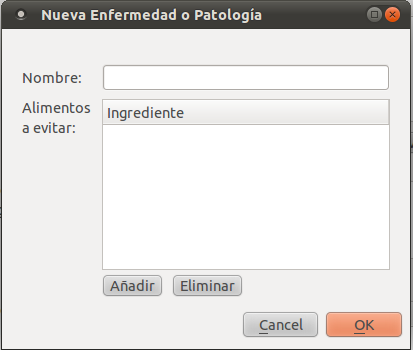
\includegraphics[scale=0.5]{Image/enfermedad-nueva.png}\\\\
Aquí se rellenará el nombre que recibe y se añadirán los ingredientes a los que afecte y se deban evitar.\\\\
\begin{itemize}
\item Añadir\\\\
Al seleccionar Añadir, se accederá a la ventana de selección de ingredientes ordenada por categorías.\\\\
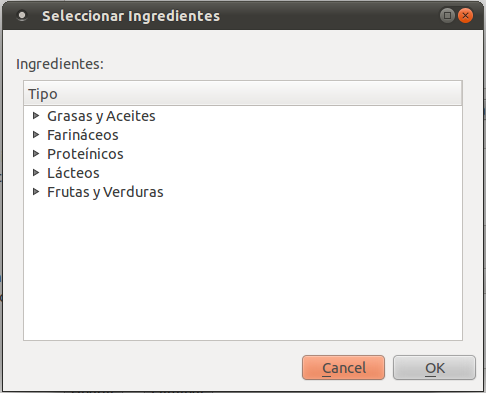
\includegraphics[scale=0.5]{Image/enfermedad-nuevoingrd.png}\\\\
\item Eliminar\\\\
Al seleccionar Eliminar, se eliminará el ingrediente seleccionado del conjunto de ingredientes a evitar.\\\\
\end{itemize}
\item Eliminar\\\\
Al seleccionar Eliminar, se eliminará tal enfermedad o patología para todos los pacientes.\\
\end{enumerate}
\item Eliminar\\\\
Al seleccionar Eliminar, se eliminará la enfermedad o patología seleccionada para dicho paciente.\\
\end{enumerate}
\end{enumerate}
\end{enumerate}




\subsubsection{Estudio Antropométrico}
Desde aquí se mostrarán los datos antropométricos, tales como peso, altura, i.m.c., peso objetivo, centímetros de cadera, centímetros de cintura, pliegue tricipital, complexión, peso ideal, peso pactado, pérdida de materia grasa, pérdida de líquidos, metabolismo basal, actividad, incremento por actividad, reducción según edad, energía total, necesidad glucídica, necesidad lipídica, necesidad proteica y tratamiento de apoyo.\\\\
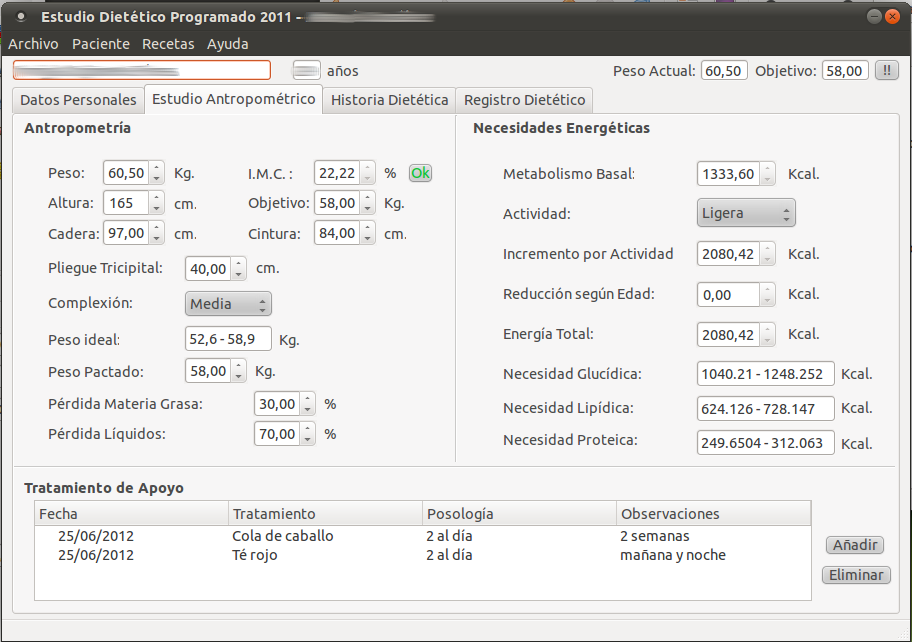
\includegraphics[scale=0.5]{Image/paciente-antrop.png}\\\\
Con estos datos se interactuará a medida de la progresión del paciente, incrementando o disminuyendo los valores, con lo que variarán algunos datos dependientes.\\
Algunos valores a tener en cuenta son:
\begin{itemize}
\item I.M.C.\\\\
Según el valor, se mostrará un indicador ofreciendo información relacionada con el mismo. al pulsarlo se mostrará una ventana con el glosario de los indicadores y su significado.\\
\item Complexión\\\\
Según sea la complexión delgada, media o ancha, variará el valor del peso ideal.\\
\item Peso Objetivo\\\\
Según el peso objetivo, variará el metabolismo basal.\\
\item Pérdida de materia grasa\\\\
Según la pérdida de materia grasa, variará la pérdida de líquidos y viceversa.\\
\item Actividad\\\\
Según sea la actividad ligera, mediana o intensa, variarán los valores del incremento por actividad, energía total, necesidad glucídica, necesidad lipídica y necesidad proteica.\\
\item Reducción según edad\\\\
Según la edad que se establece en la pestaña de datos personales, variará el valor de este indicador.\\
\item Tratamiento de Apoyo\\\\
Aquí se describirá cualquier tratamiento de apoyo que se recomiende, incluyendo su posología y observaciones si las hubiere, así como la fecha de recomendación.\\
\begin{enumerate}
\item \textit{Añadir}\\\\
Al seleccionar Añadir se accederá a la ventana para incluir un nuevo tratamiento de apoyo.\\\\
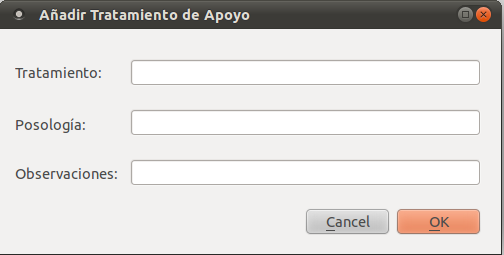
\includegraphics[scale=0.5]{Image/tratamientoAp-anadir.png}\\\\
\item \textit{Eliminar}\\\\
Al seleccionar Eliminar se eliminará el tratamiendo de apoyo seleccionado.\\\\
\end{enumerate}
\end{itemize}
\newpage




\subsubsection{Historia Dietética}
Desde aquí se tendrá acceso a las ventanas de control histórico dietético.\\\\
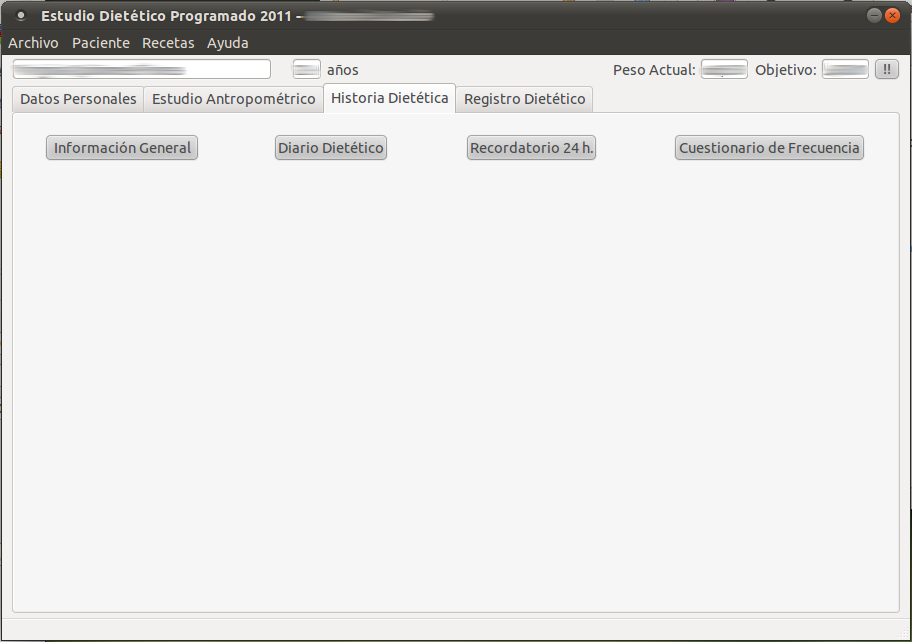
\includegraphics[scale=0.5]{Image/paciente-hist.png}\\\\
Estas ventanas se accederán mediante las opciones cuyos nombres son:
\begin{itemize}
\item Información General
\item Diario Dietético
\item Recordatorio 24h.
\item Cuestionario de Frecuencia
\end{itemize}
\newpage

\begin{enumerate}
\item \textbf{Información General}\\\\
Se trata de un cuestionario de preguntas o afirmaciones cortas, sobre las cual contestar o anotar aclaraciones, relevantes acerca de la vida del paciente, con el fin de obtener mayor información por si influenciara en alguna medida a la elaboración del semanario.\\\\
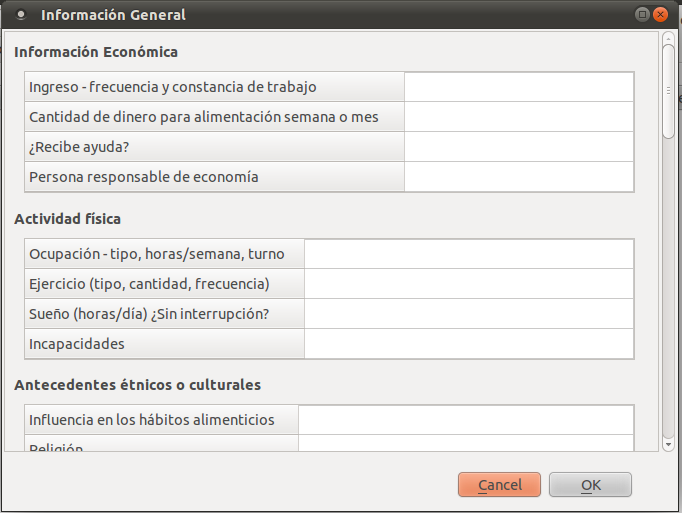
\includegraphics[scale=0.5]{Image/infogen.png}\\\\
\item \textbf{Diario Dietético}\\\\
Se trata de un registro de los recordatorios del paciente.\\\\
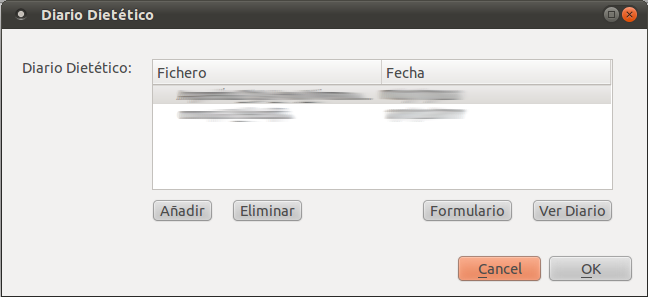
\includegraphics[scale=0.5]{Image/diariodiet.png}\\\\
También se dispone de las opciones Añadir, Eliminar, Formulario y Ver Recordatorio.
\begin{enumerate}
\item \textit{Añadir}\\\\
Al seleccionar Añadir se accederá al explorador para seleccionar un documento PDF escaneado con el recordatorio deseado.\\\\
\item \textit{Eliminar}\\\\
Al seleccionar Eliminar se eliminará del registro del paciente el recordatorio seleccionado.\\\\
\item \textit{Formulario}\\\\
Al seleccionar Formulario se accederá al diálogo de impresión para imprimir el formulario del recordatorio.\\\\
\item \textit{Ver Recordatorio}\\\\
Al seleccionar Ver Recordatorio se visualizará el recordatorio seleccionado.\\\\
\end{enumerate}
\item \textbf{Recordatorio 24h.}\\\\
Se trata de un registro de los diarios dietéticos del paciente.\\\\
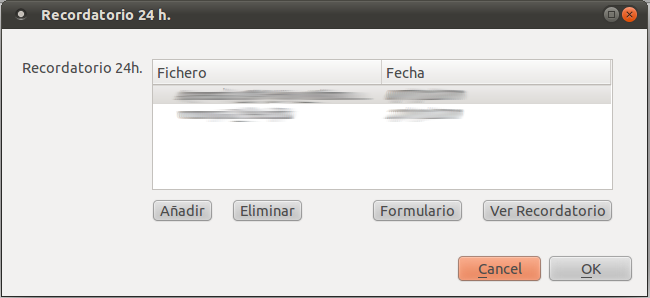
\includegraphics[scale=0.5]{Image/recordatorio.png}\\\\
También se dispone de las opciones Añadir, Eliminar, Formulario y Ver Recordatorio.
\begin{enumerate}
\item \textit{Añadir}\\\\
Al seleccionar Añadir se accederá al explorador para seleccionar un documento PDF escaneado con el diario dietético deseado.\\\\
\item \textit{Eliminar}\\\\
Al seleccionar Eliminar se eliminará del registro del paciente el diario dietético seleccionado.\\\\
\item \textit{Formulario}\\\\
Al seleccionar Formulario se accederá al diálogo de impresión para imprimir el formulario del diario dietético.\\\\
\item \textit{Ver Diario}\\\\
Al seleccionar Ver Diario se visualizará el diario dietético seleccionado.\\\\
\end{enumerate}
\item \textbf{Cuestionario de Frecuencia}\\\\
Se trata del listado de ingredientes de los cuales se podrán registrar anotaciones con la frecuencia diaria, semanal o mensual, así como la preferencia comprendida entre los valores del 1 al 5 siendo 1 el menor grador de satisfación con el ingrediente y 5 el mayor.\\\\
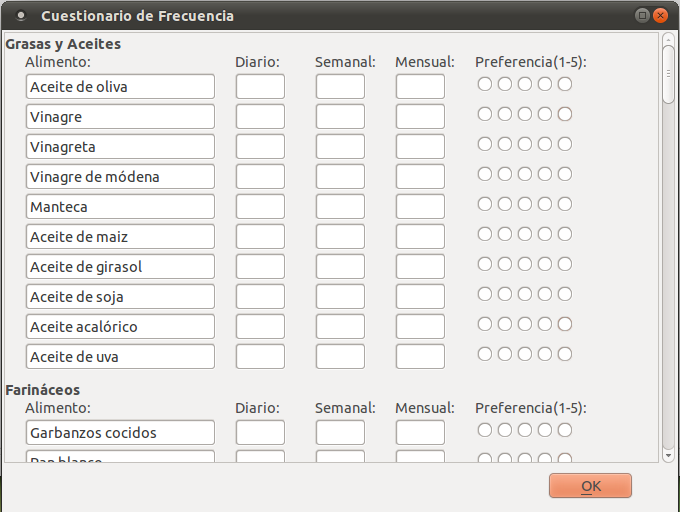
\includegraphics[scale=0.5]{Image/cuestfrec.png}
\end{enumerate}
\newpage




\subsubsection{Registro Dietético}
Desde aquí se tendrá acceso al semanario a rellenar con las recetas, así como un listado de las recetas.\\\\
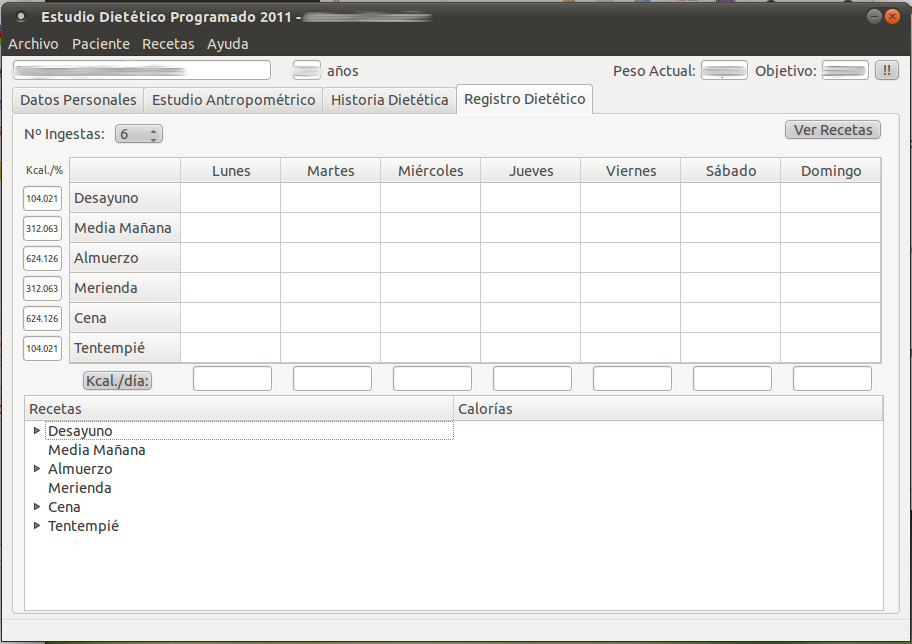
\includegraphics[scale=0.5]{Image/paciente-registro.png}\\\\
Desde el desplegable del número de ingestas, se cambiará el semanario. Siendo el mínimo posible, tres ingestas y el máximo seis ingestas. Según el número de ingestas se clasificarán como referencia en:
\begin{itemize}
\item Tres ingestas: Desayuno, Almuerzo y Cena.
\item Cuatro ingestas: Desayuno, Almuerzo, Merienda y Cena.
\item Cinco ingestas: Desayuno, Media Mañana, Almuerzo, Merienda y Cena.
\item Seis ingestas: Desayuno, Media Mañana, Almuerzo, Merienda, Cena y Tentempié.
\end{itemize}
En la parte derecha de cada comida se muestran unos indicadores con el número de kilocalorías permitidas para una de ellas.\\
El semanario se rellenará arrastrando y soltando las recetas deseadas, seleccionándolas de las recetas disponibles que se muestran.\\
En la parte inferior del semanario esta situado el botón Kcal./día, al seleccionarlo, se obtendrán los indicadores de referencia de cuántas kilocalorías tiene el día en cuestión en ese momento. Al finalizar el rellenado del semanario, se recomienda volver a pulsar dicho botón para obtener el los indicadores finales. Éstos se mostrarán en dos colores posibles, verde en el caso de ser menor a la energía total calculada en la pestaña de datos antropométricos, o en rojo en el caso de ser mayor.\\\\
Se dispone de la opción Ver Recetas, éste será un listado de las distintas recetas guardados a lo largo del seguimiento del paciente.\\\\
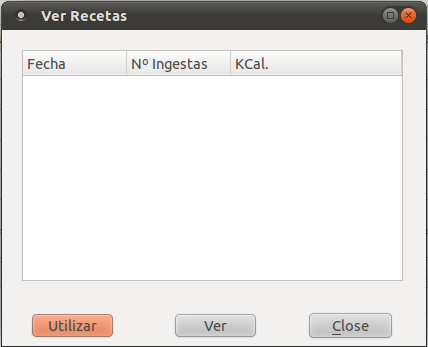
\includegraphics[scale=0.5]{Image/verrecetas.png}\\\\
En dicho listado, se clasificarán por fecha de guardado, número de ingestas y kilocalorías.\\\\
Se dispone de las opciones Utilizar y Ver.
\begin{enumerate}
\item \textit{Utilizar}\\\\
Al seleccionar Utilizar se copiarán las recetas del semanario seleccionado al actual.\\
\item \textit{Ver}\\\\
Al seleccionar Ver se abrirá un documento con el semanario seleccionado.\\
\end{enumerate}

\newpage







%%%%%%%%%%%%%%%%%%%%%%%%%%%%%%%%%%%%%%%%%%%%%%%%%%%%%%%%%%%%%%%%%%%%%%%%
\end{document}
%%%%%%%%%%%%%%%%%%%%%%%%%%%%%%%%%%%%%%%%%%%%%%%%%%%%%%%%%%%%%%%%%%%%%%%%
